\documentclass[border=10pt]{standalone}
\usepackage{tikz}
\usetikzlibrary{shapes, positioning, decorations.pathreplacing, fit}
% Includes shared by multiple tex files
\usepackage{xcolor}
\definecolor{primary}{RGB}{170,0,255}
\definecolor{secondary}{RGB}{255,177,25}
\definecolor{ternary}{RGB}{20,204,113}
\definecolor{win}{RGB}{20,255,20}
\definecolor{lose}{RGB}{255,20,20}
\definecolor{faded}{gray}{0.5}
\definecolor{invis}{gray}{0.9}


\begin{document}
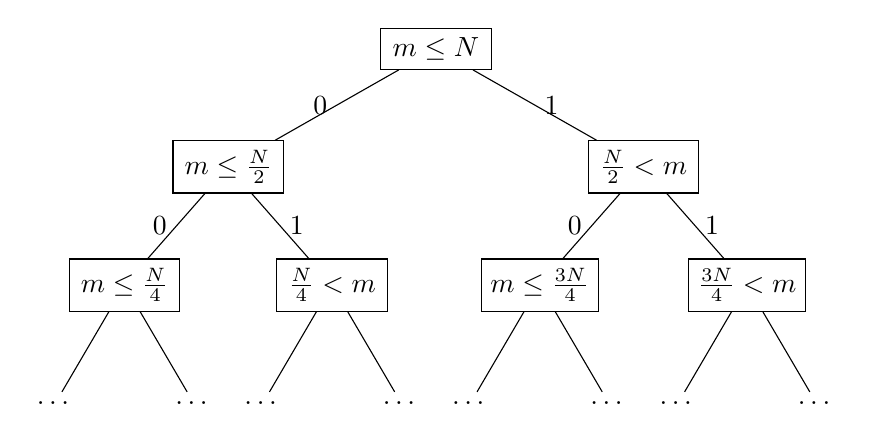
\begin{tikzpicture}[level/.style={sibling distance=15em/#1}]

  \tikzstyle{bound} = [rectangle, draw, align=center, minimum width=4em];
  \node[bound] (root) {$m \leq N$}
    child {
      node[bound] {$m \leq \frac{N}{2}$}
      child {
        node[bound] {$m \leq \frac{N}{4}$}
        child { node {\dots}}
        child { node {\dots}}
        edge from parent node[left] {0}
      }
      child {
        node[bound] {$\frac{N}{4} < m$}
        child { node {\dots}}
        child { node {\dots}}
        edge from parent node[right] {1}
      }
      edge from parent node[left] {0}
    }
    child {
      node[bound] {$\frac{N}{2} < m$}
      child {
        node[bound] {$m \leq \frac{3 N}{4}$}
        child { node {\dots}}
        child { node {\dots}}
        edge from parent node[left] {0}
      }
      child {
        node[bound] {$\frac{3 N}{4} < m$}
        child { node {\dots}}
        child { node {\dots}}
        edge from parent node[right] {1}
      }
      edge from parent node[right] {1}
    };
\end{tikzpicture}
\end{document}
